\chapter{Using and Modifying the Data Structure}
\label{chapter:data_structure}
MAUS operates on data in discrete blocks, primarily spills, with one spill representing the particle burst generated by one dip of the MICE target. Additionally, MAUS can write data into a JobHeader, RunHeader, RunFooter and JobFooter data type. Histograms for plotting in online mode are encoded into an Image data type. The top level branch in the data tree inherits from MAUSEvent<T>, defined in \verb|src/common_cpp/DataStructure/MAUSEvent.hh| (C++) with type identified by GetEventType() string; in JSON the top level branch always has a \verb|maus_event_type| member which is a string value corresponding to the output of MAUSEvent<T>::GetEventType(). A summary of configuration cards affecting Input, Output and data structure is shown below.

\begin{table*}
\begin{center}
\caption{I/O control variables.}
\begin{tabularx}{\linewidth}{lX}
Name & Meaning \\
\hline
\verb|input_root_file_name| & Set the file name used for reading input files by InputCppRoot module \\
\verb|output_root_file_name| & Set the file name used for writing output files by OutputCppRoot module  \\
\hline
\verb|input_json_file_name| & Set the file name used for reading input files by InputPyJSON module \\
\verb|input_json_file_type| & Set to \verb|gzip| to read input from a gzipped file; set to \verb|text| to read input from a plain text file \\
\verb|output_json_file_name| & Set the file name used for writing output files by OutputPyJSON module \\
\verb|output_json_file_type| & Set to \verb|gzip| to write output as a gzipped file; set to \verb|text| to write output as a plain text file  \\
\hline
\verb|header_and_footer_mode| & Set to \verb|append| to write out job and run headers and footers; set to \verb|dont_append| to suppress this output. \\
\begin{makeimage} % force latex2html to render as an html table 
\end{makeimage} 
\end{tabularx}
\end{center}
\end{table*}

\section{Metadata}
Job metadata is stored in JobHeader and JobFooter data structures. (Data) Run metadata is stored in RunHeader and RunFooter data structures. The JobHeader is created at the start and end of an execution of the code and stores data on datacards, bzr state and so forth. The RunHeader is created at the start of each run and stores per run metadata such as the calibrations and cablings used. One RunHeader and RunFooter is written for each process in the entire \emph{transform} and \emph{merge} execution structure; so in multithreading mode this would yield one RunHeader and RunFooter for each Celery subprocess (which runs the Input/Transform) and an additional RunHeader and RunFooter for the merge/output process. In single threaded mode a single RunHeader and RunFooter is generated. The RunFooter and JobFooter are created at the end of the run and store run and job summary information. For more details on writing to these metadata types and multithreading modes, please see the section on API.

The Metadata is stored in ROOT in trees separate to the main Spill data tree. In JSON, these data are stored as separate lines often at the start and end of the run, and distinguished by the \verb|maus_event_type| branch in the root. The structure of a MAUS output file is shown below.

\begin{figure}[!htb]
\centering
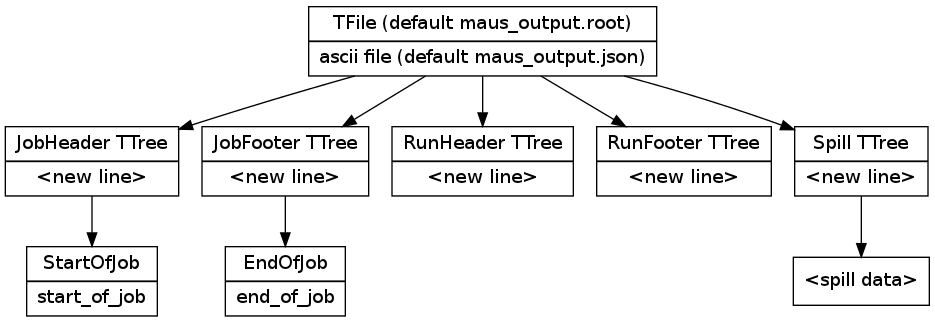
\includegraphics[width=0.9\textwidth]{file_structure.png}
\caption{The MAUS file structure including metadata. The top label in each box describes the representation in C++/ROOT. The bottom label describes the representation in JSON.}
\end{figure}


\section{The Spill Datastructure}
The major part of the MAUS data structure therefore is a tree of which each entry corresponds to the data associated with one spill. The spill is separated into three main sections: the MCEventArray contains an array of data each member of which represents the Monte Carlo of a single primary particle crossing the system; the ReconEventArray contains an array of data each member of which corresponds to a particle event (i.e. set of DAQ triggers); and the DAQData corresponds to the raw data readout. Additionally there are branches for reconstructed scalars, which are handled spill by spill and EMR data, which also read out on the spill rather than event by event.

\begin{figure}[!htbp]
\centering
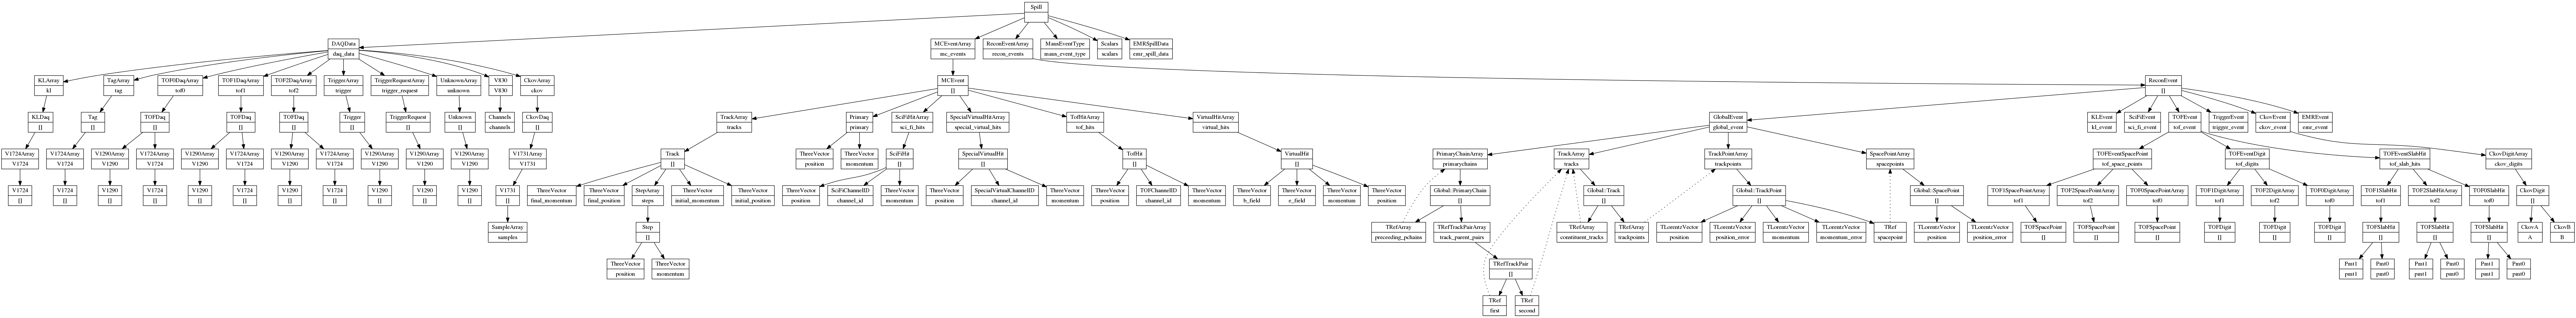
\includegraphics[width=0.9\textwidth]{spill_structure.png}
\caption{The MAUS output structure for a spill event. The top label in each box is the name of the C++ class and the bottom label is the json branch name. If a [] is shown, this indicates that child objects are array items.}
\end{figure}

The MCEvent is subdivided into sensitive detector hits and some pure Monte Carlo outputs. The primary that led to data being created is held in the Primary branch. Here the random seed, primary position momentum and so forth is stored. Sensitive detector hits have Hit data (energy deposited, position, momentum, etc) and a detector specific ChannelId that represents the channel of the detector that was hit - e.g. for TOF this indexes the slab, plane and station. Virtual hits are also stored - these are not sensitive detector hits, rather output position, momenta etc of particles that cross a particular plane in space, time or proper time is recorded. Note virtual hits do not inherit from the Hit class and have a slightly different data structure.

The ReconEvent and DAQEvents are subdivided by detector. ReconEvents contain reconstructed particle data for each detector and the trigger. There is an additional branch that contains global reconstruction output, that is the track fitting between detectors.

The data can be written in two formats. The main data format is a ROOT binary format. This requires the ROOT package to read and write, which is a standard analysis/plotting package in High Energy Physics and is installed by the MAUS build script. The secondary data format is JSON. This is an ascii data-tree format that in principle can be read by any text editor. Specific JSON parsers are also available - for example, the python \emph{json} module is available and comes prepackaged with MAUS.

\section{Image Datastructure}
There is a final data type that MAUS handles, the Image type. The Image data structure is written by ReducePyMatplotHistogram and ReducePyROOTHistogram data types. Image data is only available in JSON format. The data structure is shown in Fig. \ref{fig:image-structure}.

\begin{figure}[!htb]
\centering
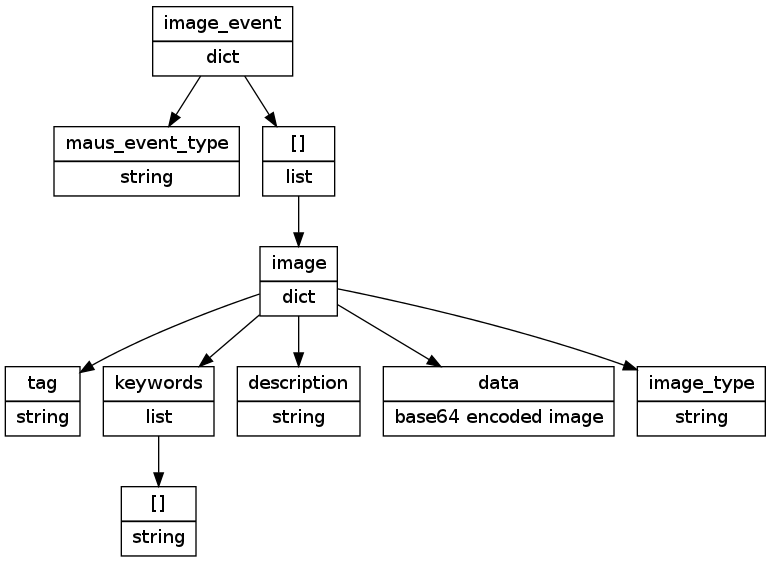
\includegraphics[width=0.9\textwidth]{image_structure.png}
\label{fig:image-structure}
\caption{The MAUS output structure for an Image event. The top label in each box is the name of the JSON branch and the bottom label is the data type. If a [] is shown, this indicates that child objects are array items. Note there is no C++ implementation of Image events}
\end{figure}

Each document contains a \verb|maus_event_type| that should always be \verb|Image|, and a list of images; the image data is encoded as a base 64 image and other data associated with the image is stored alongside. The \verb|tag| names the image, while \verb|image_type| describes the data format (png, jpeg, etc). OutputPyImage stores data with \verb|image_type.tag| as the file name.  \verb|description| contains a description of the file and keywords describes a list of key phrases that can be used when searching. 

\section{Accessing ROOT files}
For details on how to access the ROOT files, please see the introduction section of this document.

\section{Conversion to, and Working With, JSON}
MAUS also provides output in the JSON data format. This is an ascii format with IO libraries available for C++, Python and other languages. Two utilities are provided to perform conversions, \verb|bin/utilities/json_to_root.py| and \verb|bin/utilities/root_to_json.py| for conversion from and to JSON format respectively. JSON Input and Output modules are provided, \verb|InputPyJson| and \verb|OutputPyJson|.

An example json analysis is available in \verb|bin/examples/load_json_file.py|/

\section{Extending the Data Structure}
The data structure can be extended in MAUS by adding extra classes to the existing data structure. The data classes are in \verb|src/common_cpp/DataStructure|. In order to make these classes accessible to ROOT, the following steps must be taken:
\begin{itemize}
\item Add a new class in \verb|src/common_cpp/DataStructure|.
\item Ensure that default constructor, copy constructor, equality operator and destructor is present. The destructor must be virtual.
\item Add \verb|#include "src/common_cpp/Utils/VersionNumber.hh"| and a call to the \verb|MAUS_VERSIONED_CLASS_DEF()| macro at the end of the class definition before the closing braces. \verb|MAUS_VERSIONED_CLASS_DEF| calls the ROOT ClassDef() macro which generates metaclasses based on information in the class. This is put into the (dynamically generated) \verb|MausDataStructure.h,cc| files.
\item Add the class to the list of classes in \verb|src/common_cpp/DataStructure/LinkDef.hh|. This is required for the class to be linked properly to the main library, and a linker error will result if this step is not taken.
\item Add any template definitions which you used, including STL classes (e.g. std::vector<MyClass> or whatever) to linkdef. Otherwise ROOT will generate a segmentation fault whenever the user tries to call functions of the templated class (but the code will link successfully in this case).
\end{itemize}
In order to make these classes accessible to JSON, it is necessary to add a new processor in \verb|src/common_cpp/JsonCppProcessors|. There are a few default processors available.
\begin{itemize}
\item \verb|src/common_cpp/JsonCppProcessors/ProcessorBase.hh| contains IProcessor pure interface class for all processors and ProcessorBase base class (which may contain some implementation)
\item \verb|src/common_cpp/JsonCppProcessors/PrimitivesProcessors.hh| contains processors for primitive types; BoolProcessor, IntProcessor, UIntProcessor, StringProcessor, DoubleProcessor
\item \verb|src/common_cpp/JsonCppProcessors/ArrayProcessors.hh| contains processors for array types. Two processors are available: PointerArrayProcessor which converts an STL vector of pointers to data; and ValueArrayProcessor which converts an STL vector of values to data.
\item \verb|src/common_cpp/JsonCppProcessors/ObjectProcessor.hh| contains a processor for object types. Most of the classes in the MAUS data structure are represented in JSON as objects (string value pairs) where each string names a branch and each value contains data, which may be another class.
\item \verb|src/common_cpp/JsonCppProcessors/ObjectMapProcessors.hh| contains a processor for converting from JSON objects to STL maps. This is useful for JSON objects that contain lots of branches all of the same type.
\end{itemize}

A script, \verb|bin/user/json_branch_to_data_structure_and_cpp_processor.py| is available that analyses a JSON object or JSON tree of nested objects and converts to C++ classes. The script is provided "as-is" and it is expected that developers will check the output, adding comments and tests where appropriate.

\subsection{Pointer Handling}
MAUS can handle pointers for arrays and classes using ROOT native support
(via the \verb|TRef| and \verb|TRefArray| classes)
or the standard JSON reference syntax. 
JSON references are indexed by a path relative to the root value of a JSON document. 
JSON references are formatted like URIs, 
for example the JSON object \verb|{"$ref":"#spill/recon_events/1"}| 
would index the second \verb|recon_event| in the spill object (indexing from 0). 
MAUS can only handle paths relative to the top level of the JSON document for the same MAUS event. 
Absolute URIs, URIs relative to another position in the JSON document or URIs to another MAUS event are not supported. 

In MAUS, it is necessary to make a distinction between data that is stored as a value in C++ and JSON (value-as-data), 
data that is stored as a pointer in C++ and a value in JSON (pointer-as-data) 
and data that is stored as a pointer in C++ and JSON to some other data in the same tree (pointer-as-reference). 
In the latter case, the C++ parent object does not own the memory; 
rather it is owned by some other object in the same tree and 
\emph{borrowed} by the C++ object holding the pointer-as-reference.
The \verb|TRef| and \verb|TRefArray| classes provide this functionality by default;
never owning the memory but only storing a relevant pointer.
All objects referenced by a \verb|TRef| or \verb|TRefArray|
must inherit from \verb|TObject|.
ROOT handles all memory management while writing to and reading from ROOT files,
and the order of reading is unimportant,
as long as both reference and value have been read before the reference is used.

Pointers-as-data are converted between JSON arrays and C++ objects
using the \verb|ObjectProcessor<ParentType>::RegisterPointerBranch<ChildType>| method.
This takes a Processor for the ChildType as an argument.
For C++ arrays / vectors, the Processor argument is instead a 
\verb|PointerArrayProcessor<ArrayContents>|.
Pointers-as-reference (TRef and TRefArray) are converted using the
\verb|ObjectProcessor<ParentType>::RegisterTRef| and 
\verb|ObjectProcessor<ParentType>::RegisterTRefArray| methods respectively.

Other equivalent data formats, for example YAML, use a unique identifier to reference a pointer-as-reference and store the pointer-as-data in a reserved part of the data tree. There are some consequences of storing pointers-as-reference using the path to a pointer-as-data as implemented in MAUS.
\begin{itemize}
\item The user must specify which data is the primary data source (pointer-as-data) and which data is a cross reference (pointer-as-reference).
\item Pointers-as-reference are position dependent. If the associated pointer-as-data is moved the pointer-as-reference can no longer be resolved. For example, inserting an element into an array can cause misalignment of pointers-as-reference.
\item Pointer data will always be available at the location of the pointer-as-data in the JSON tree, even when using a parser that is not pointer aware.
\item A unique identifier type algorithm can be implemented as a relatively simple extension of the data format outlined here; but it is relatively hard to extend a unique identifier algorithm to reference existing parts of the data tree.
\end{itemize}

\subsubsection{Pointer Resolution}
Conversion from C++ pointers to JSON pointers is handled in a type-safe way. Values-as-data are stored in the data tree converted at run time from JSON to C++ and vice versa. Pointers-as-data are handled in the same way as Values-as-data. Pointers-as-references are stored in the C++ data tree as a TRef (or TRefArray element) in the normal way, and in JSON as an address to the position in the tree to a pointer-as-data. It is an error to store a pointer-as-reference without storing an associated pointer-as-data as the pointer-as-reference cannot be converted, unless the pointer-as-reference is set to NULL (in which case it may be an error depending on caller settings). It is an error to store multiple C++ pointers-as-data to the same memory address as the conversion from C++ to JSON and back again would yield logically different data and the resolution of associated pointers-as-reference is dependent on the resolution order of the data tree, which is ill-defined.

In order to implement the data conversion, the pointers have to be resolved in a two-stage process. In the first stage, it is necessary to collect all of the pointers-as-data and pointers-as-reference by traversing the data tree. This is performed during the standard data conversion, but pointers-as-reference are left pointing to NULL. A mapping from the pointer-as-data in the original data format to the pointer-as-data in the converted data format is stored, together with a list of pointers-as-reference in the original data format and the necessary mutators in the converted data format. In the second stage MAUS iterates over the pointers-as-reference, finds the appropriate pointer-as-data and writes the location of the pointer-as-data to the pointer-as-reference in the converted data format. The code is templated to maintain full type-safety during this process.
 
